%--------------------------------------------------------
% S3. Vectors d'eucariotes
%--------------------------------------------------------

\section{Vectors d'eucariotes}
\label{sec:vectors-deucariotes}

L'interès de clonar en organismes eucariotes té sentit per obtenir proteïnes amb les modificacions post-traduccionals correctes o bé per estudiar processos biològics en eucariotes.

Un altre problema és l'ús de codons. Com que el codi genètic està degenerat, i no té perquè ser compartit per tots els organismes ni la freqüència dels codons/anticodons és la mateixa.

\subsection{Vectors de llevats}
\label{sec:vectors-de-llevats}
En\textit{Saccharomyces cerevisiae}, hi ha soques que tenen un plàsmid de 6 kb. El sistema de selecció en eucariotes és l'auxotròfia (deficiència en biosíntesi d'un aminoàcid), i per això s'han aïllat soques de Saccharomyces auxotrofes per diferents aminoàcids. Els vector inclouen el gen que està mutat en aquestes soques, de manera que els transformants podran créixer en medi selectiu per aquest element en concret.

Shuttle vector: és un vector que pot actuar en 2 organismes diferents. El que es va fer va ser juntar 2 vectors (pRB322 i un plàsmid de llevats), de manera que repliquin en E. coli i Saccharomyces.

\begin{itemize}
\item YEPS: \textit{Yeast Episomal plasmid}. Es pot integrar mitjançant recombinació homòloga.
\item YIPS: \textit{Yeast Integrative plasmid}. Sempre s'integren al genoma del llevat.
\item YRPS: \textit{Yeast Replicative plasmid}. Mai s'integren al genoma.
\end{itemize}

Un episoma és una seqüència que pot estar integrada al cromosoma bacterià o en forma de plàsmid.

\subsection{YAC}
\label{sec:yac}
Els YAC són \textit{Yeast Artificial Chromosome}. Els fragments més grans de 40 kb són molt difícils de clonar. Els YAC permetien clonar fins a 600 kb. Són molt inestables i recombinen molt.

Els YACs són els vectors de clonatge més utilitzats, ja que són els que accepten més material genètic. Són vectors duals, ja que poden adquirí forma de plasmidi o de cromosoma eucariota típic, lineal.

En una primera etapa aquest cromosoma es troba en una conformació circular; encara no ha incorporat l'insert de DNA que volem clonar. Es transformen bacteris amb aquests YACs, que funcionen com a plasmidi bacterià, ja que tenen el Ori bacterià, i es replica dins aquests. Després s'introduiran a cèl·lules de llevat.

Els YACs tenen un marcador de resistència a l'ampicil·lina (Amp), el que ens permet identificar quines cèl·lules han incorporat aquest vector. Contenen també altres elements eucariotes, com ara telòmers de llevat (TEL), el centròmer (CEN4), l'origen de replicació de llevat (ARS1), i gens marcadors de cèl·lules eucariotes, com TRP1 i URA3.

Quan aquests plasmidis es digereixen, s'obtenen dues molècules, corresponents al braç llarg i al braç curt del cromosoma, els quals s'uneixen per formar el cromosoma eucariota comú mitjançant una lligasa. És en el moment en el que utilitzem aquesta lligasa quan incorporem el DNA digerit que volem mapar.

L'enzim que digereix el YAC és el mateix que realitza la digestió parcial del nostre DNA.

Els dos marcadors esmentats, TRP1 i URA3, es troben al braç llarg i al braç curt respectivament. TRP1 és necessari per a la síntesi de triptòfan, i URA3 és un enzim de la via biosintètica de l'uracil. Aquests dos marcadors ens són útils, ja que utilitzem cèl·lules que no poden sintetitzar triptòfan ni uracil per si soles per tal de comprovar que incorporin el YAC. El medi, doncs, tampoc tenen aquests compostos.

Per assegurar que l'insert del DNA que volem mapar ha anat bé, necessitem un tercer marcador, SUP4, que es troba en el lloc de digestió del plasmidi i, per tant, en el lloc de l'insert del DNA. Si el DNA problema s'incorpora correctament al YAC, el gen SUP4 queda partit, dividit; però si l'insert no s'ha incorporat correctament, el gen SUP4 romandrà intacte.

El gen SUP4 codifica per un tRNA especial que reconeix el codó de STOP però que incorpora un aminoàcid, fet que no és normal en els tRNA que reconeixen codons d'aturada. D'aquesta manera que obtindrem proteïnes més llargues del que és normal, ja que allà on hi hagi un codó STOP hi seguirà havent un aminoàcid i la transcripció continuarà.

Així doncs tenim que les cèl·lules de llevat són triples mutants: no sintetitzen triptòfan, no sintetitzen uracil i tampoc sintetitzen adenina. Al no sintetitzar adenina, el seu precursor de la ruta bioquímica s'acumula, i dóna una tonalitat vermellosa a la cèl·lula.

El medi no incorporarà triptòfan ni uracil, però si es posa una quantitat d'adenina limitant, ja que sinó les cèl·lules no serien viables.

En afegir un cromosoma amb SUP4 funcional, la ruta de síntesi de l'adenina funcionarà correctament, ja que un dels enzims mutats de la via biosintètica d'aquest nucleòtid presenta un codó STOP, i al afegir el tRNA de SUP4 aquest codó STOP serà obviat (s'afegirà un aminoàcid igualment) i l'enzim serà funcional. Aleshores el precursor que dóna la tonalitat vermellós a no s'acumularà i veurem la cèl·lula amb una tonalitat blanquinosa.

D'aquesta manera:
\begin{itemize}
\item Si no s'insereix correctament el nostre DNA d'interès al YAC, el gen SUP4 queda intacte, es sintetitza el tRNA corresponent i es duu a terme una correcta síntesi d'adenina, donant a la cèl·lula una tonalitat blanquinosa.

\item Si s'insereix correctament el nostre DNA d'interès al YAC, el gen SUP4 queda fraccionat i no és funcional, pel què no existeix el tRNA corresponent i no es sintetitzarà adenina, fent que s'acumuli el seu precursor i donant a la cèl·lula una tonalitat vermella.
\end{itemize}

Això, però, ens suposa un problema, ja que el tRNA de SUP4 farà que qualsevol codó STOP normal no tingui el seu ús habitual; les cèl·lules seguiran sent viables però les proteïnes tindran una longitud major.

\subsubsection{Estratègia de clonatge amb YACs} \hfill \\
\begin{itemize}
\item \textbf{Soca AB1380:} contenen URA3, TRP1 i ade2.1. L'al·lel ade2.1 provoca un bloqueig en la síntesi de l'adenina, causant un cúmul de pigment vermell a la cèl·lula. És suprimible per SUP4.
\item \textbf{pYAC:} contenen URA3, TRP1 i SUP4.
\item \textbf{Soca AB1380 que conté el vector pYAC sense insert:} observem colònies blanques, ja que SUP4 suprimeix la mutació ade2.1.
\item \textbf{Soca AB1380 que conté el vector pYAC amb insert:} observem colònies vermelles, ja que l?insert inactiva el supressor SUP4.
\end{itemize}

\begin{figure}[H]
\centering
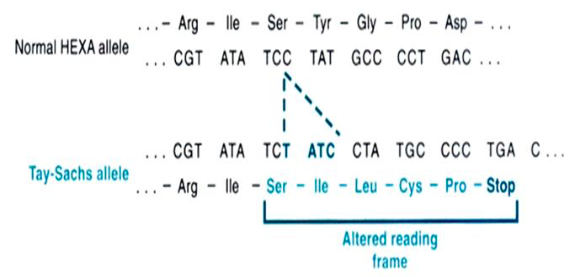
\includegraphics[width=0.8\textwidth]{fig17}
\end{figure}

\subsubsection{Inconvenients dels YACs}
Els YACs són molècules inestables i poden esdevenir quimèrics degut a la gran mida dels inserts. Són grans fonts de reordenaments, com per exemple delecions de seqüències Alu reconegudes per homologia.

Normalment tenim tot el genoma en una barreja de lligació i es posa en contacte amb cèl·lules de llevat, incorporant cadascuna un sol insert. Es plaqueja de forma que cada cèl·lula de la nostra solució estigui prou separada de la resta com per formar colònies d'un sol vector. Pot passar, però, que durant la lligació s'incorporin dos inserts en un sol vector, obtenint un vector quimera. Això ens causarà dificultats en el moment del reordenament del genoma.

Els YACs tenen un 15-20\% de quimerisme.

Amb l'ús d'altres vectors, com BACs o PACs, perdem capacitat, però el quimerisme i la inestabilitat deixaran de ser un problema.

\subsection{Vectors per plantes}
\label{sec:vectors-de-plantes}
Els vector de plantes i animals es basen en genomes vírics. Els vectors derivats del plàsmid Ti. \textit{Agrobacterium tumefaciens} transfereix el plàsmid a la cèl·lula de la planta i després el plàsmid s'integra al genoma de la planta. S'indueix la proliferació cel·lular i s'activa la síntesi de compostos que són d'aliment per \textit{A. tumefaciens}. El problema és que Ti és molt gran i és molt complicat clonar un fragment. El que s'ha fet és dividir el plàmid en 2: una part que conté les funcions del plàsmid i un altre que conté les regions per transferir el gen a la planta.

\subsection{Vectors per mamífers}
\label{sec:vectors-per-mamifers}
